%!TEX root = ./report.tex
\section{Background}
\label{background}

In this section, we provide some background information on Fortune's algorithm for generating Voronoi diagrams, and the trapezoidal map algorithm for point location, which we will later merge into one.

\subsection{Fortunes Algorithm}
Fortune’s algorithm is a sweep line algorithm that generates a Voronoi diagram from a set of sites given as input. By sweeping a horizontal line from top to bottom of all the sites the algorithm is capable of determining the position of all vertices and edges in the diagram. The output is a doubly connected edge list (DCEL) corresponding to the edges of a Voronoi diagram.

\paragraph{}
In general, the edges of a Voronoi diagram can be full lines, meaning that they have one or zero endpoints, or they can be true line segments. To be able to store the edges of the result in a DCEL, the algorithm outputs all edges as segments. This is achieved by assuming that all sites are contained in a bounding rectangle that cuts off the lines that would otherwise be unbounded.

To compute the diagram, the algorithm sweeps from the top of the rectangle and terminates when it reaches the bottom. During the sweep, two kinds of events can happen. 

\subsubsection{Site events}
occur when the sweep line reaches a new site. After a site event it is possible to define a parabola with its narrow end pointing downwards, and the site that caused the event as its focal point. When this happens, all the points that lie inside the parabola will be closer to the newly discovered site than to any other site lying below the sweep line. As soon as the sweep line reaches the next site, a new parabola will be created and so on. A snap shot of the algorithm in progress can be seen in Figure~\ref{fig:fortunes}.

\begin{figure}[]
    \centering
      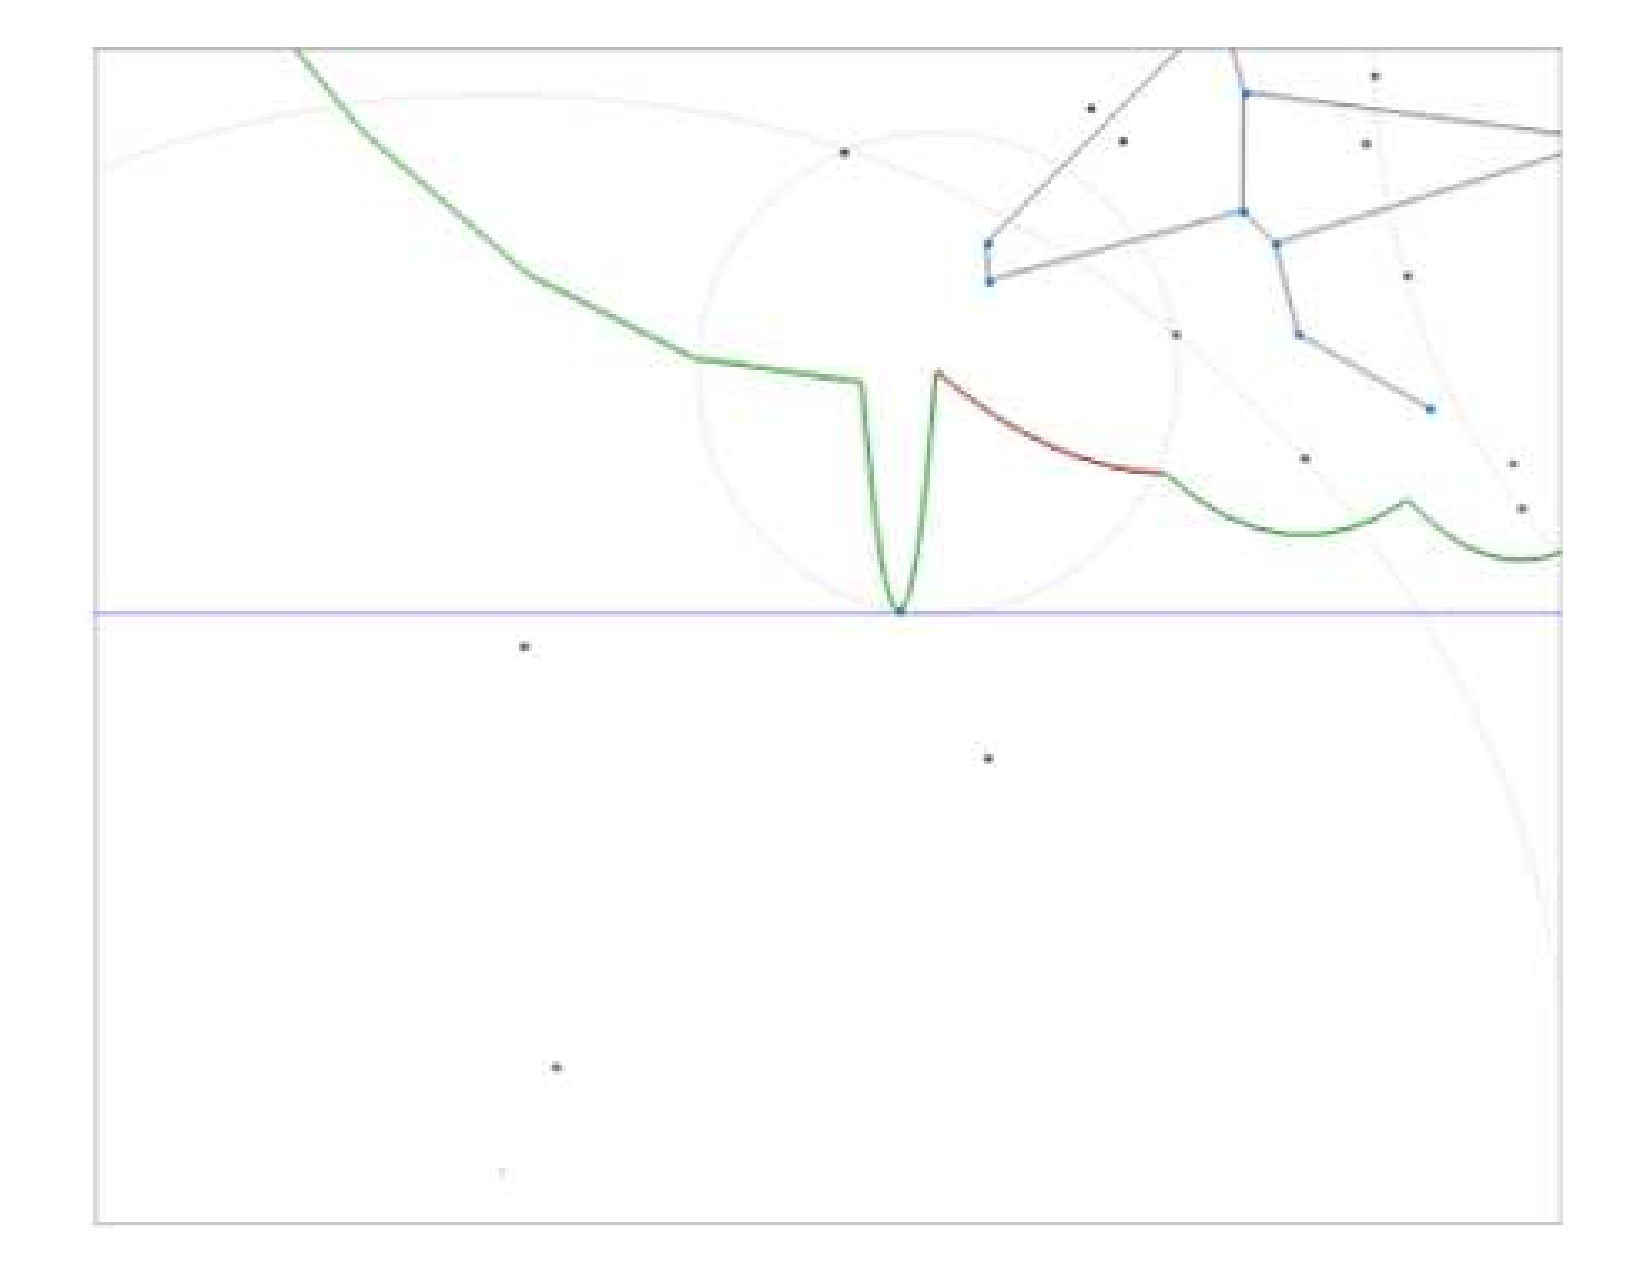
\includegraphics[width=80mm]{images/fortunes.pdf}
    \caption{Snapshot of Fortune's algorithm. A site event has just occured on the sweep line, and a few line segments and vertices have been discovered in the upper right corner. Below the sweep line we see 3 future site events.}
    \label{fig:fortunes}
\end{figure}

\paragraph{}
Since the points that form the intersections between two parabolas are equidistant to the sites represented by their respective parabolas, these intersections must be part of the final Voronoi diagram, by definition. Since the size of the parabolas depend on the location of the sweep line, they will widen as the sweep line advances its position. The intersections will move as well and trace out the line segments of the Voronoi diagram. Initially, when the sweep line is in the horizontal position of the new site, the parabola is just a vertical line crossing the site.

\subsubsection{Circle events}
occur when the sweep line reaches a position where it acts as a horizontal tangent to a circle that also intersects three sites above the sweep line. At that moment, a situation has occurred where three points with known positions are equidistant to the centre of the circle. Since the centre of the circle is equidistant from more than two points, it becomes a vertex in the Voronoi diagram. The situation is shown in Figure~\ref{fig:circle_event}.

\begin{figure}[]
    \centering
      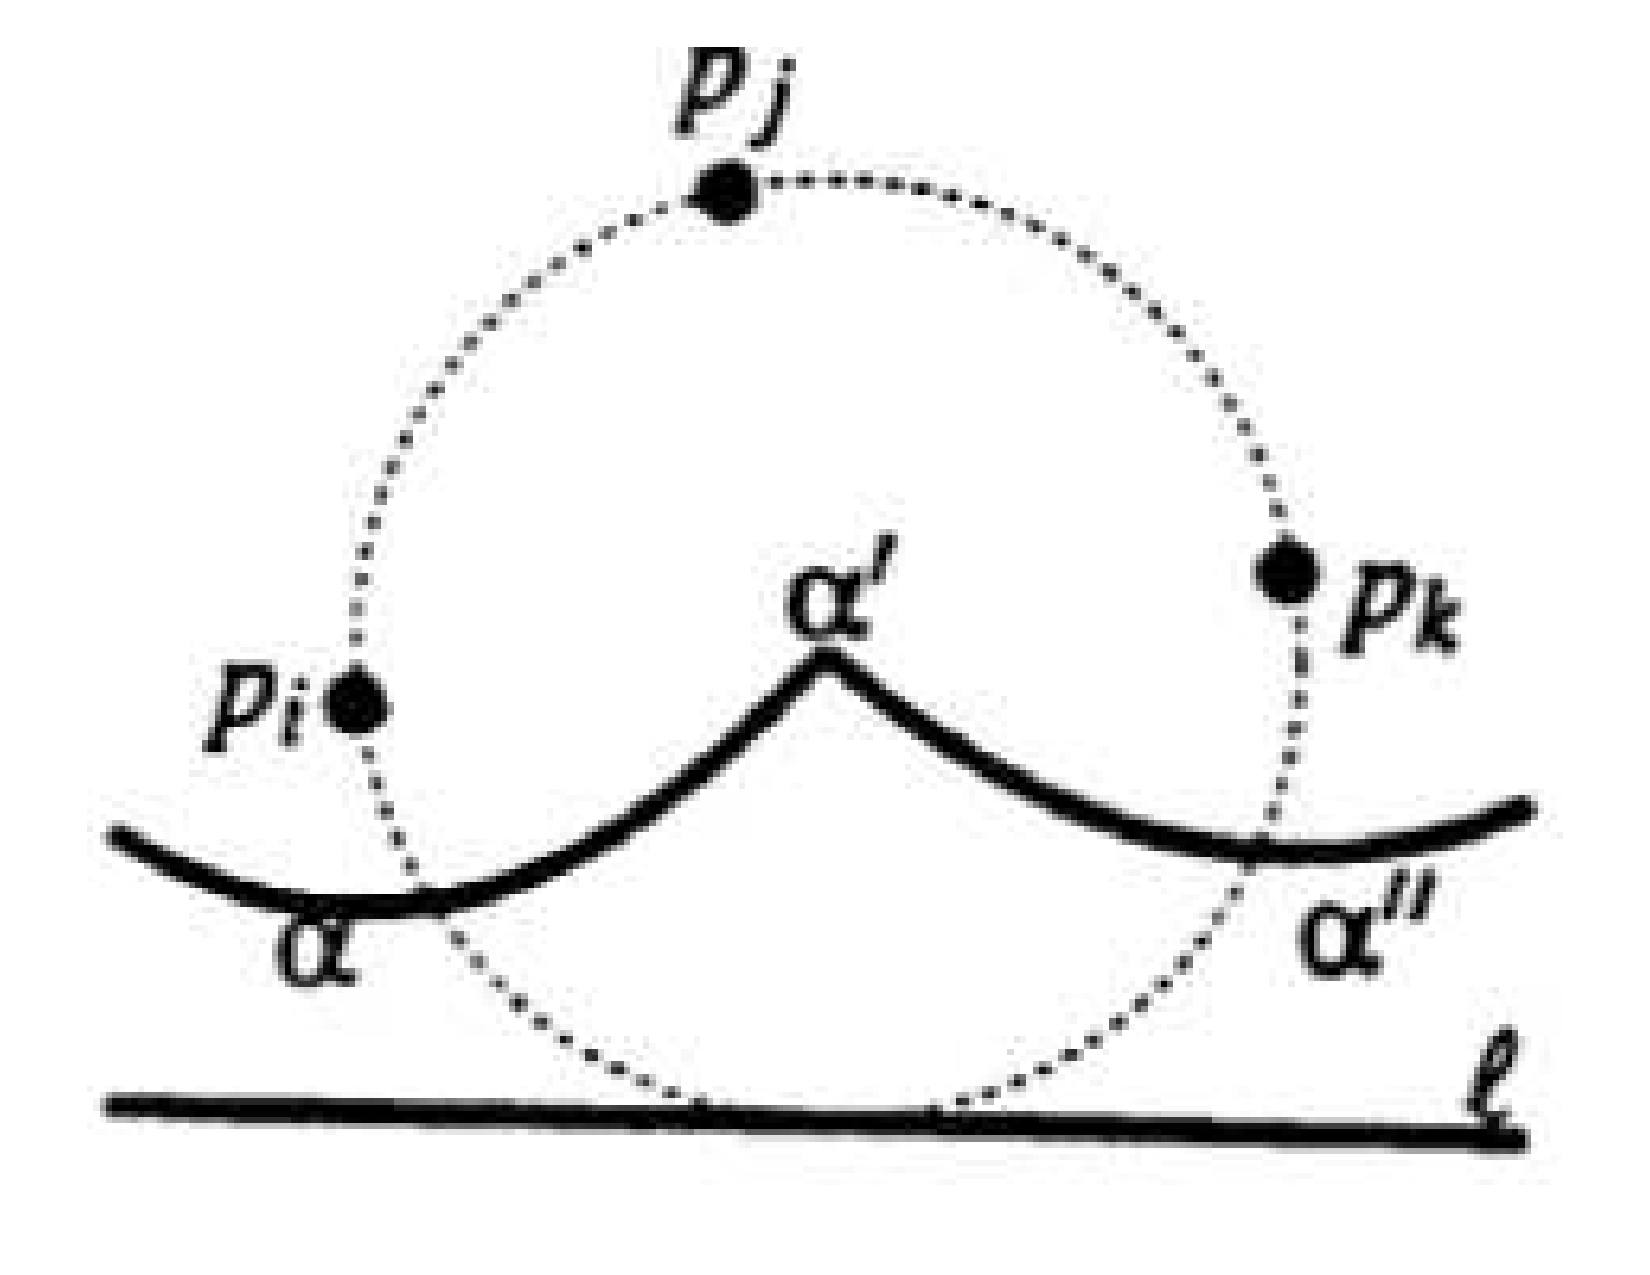
\includegraphics[width=50mm]{images/circle_event.pdf}
    \caption{Circle event. A circle with sites $pi$, $pj$ and $pk$ on its perimiter is tangent on the sweep line $l$, and a vertex $a'$  has been discovered in its centre.}
    \label{fig:circle_event}
\end{figure}

During the sweep, the algorithm maintains a so-called beach line. This is the curvy line just above the sweep line seen in Figure~\ref{fig:fortunes}. For each x coordinate the beach line consists of the lowest y value of any parabola. This means that the beach line consists of parabolic arcs, where each parabola can contribute to the beach line more than once.

It turns out that a circle event happens exactly when an arc of the beach line disappears because it is hidden by two neighbouring arcs. These two arcs will grow faster than a third arc, that ultimately degenerates to a single point, which forms the centre of the circle mentioned above.

\subsection{Point Location}
\subsubsection{Single Shot Algorithm}
The single shot algorithm takes as input a set of line segments forming a planar sub division. It answers queries of the same type as the point location algorithm to be explained in the next section but has a time complexity of O(n) meaning that it is not optimal. 

\paragraph{}
Basically, what the algorithm does is to locate the line segment lying directly below the query point in the cell. If the segments are stored in a DCEL, the segment that was found can then be used to trace out the rest of the cell. To find the segment, the algorithm runs through the whole list and iteratively tries to find a better candidate by looking at the coordinates of the end points. An optimal (and valid) candidate will lie below the query point and be closer to it than any other segment lying below it. 

\begin{figure}[]
    \centering
      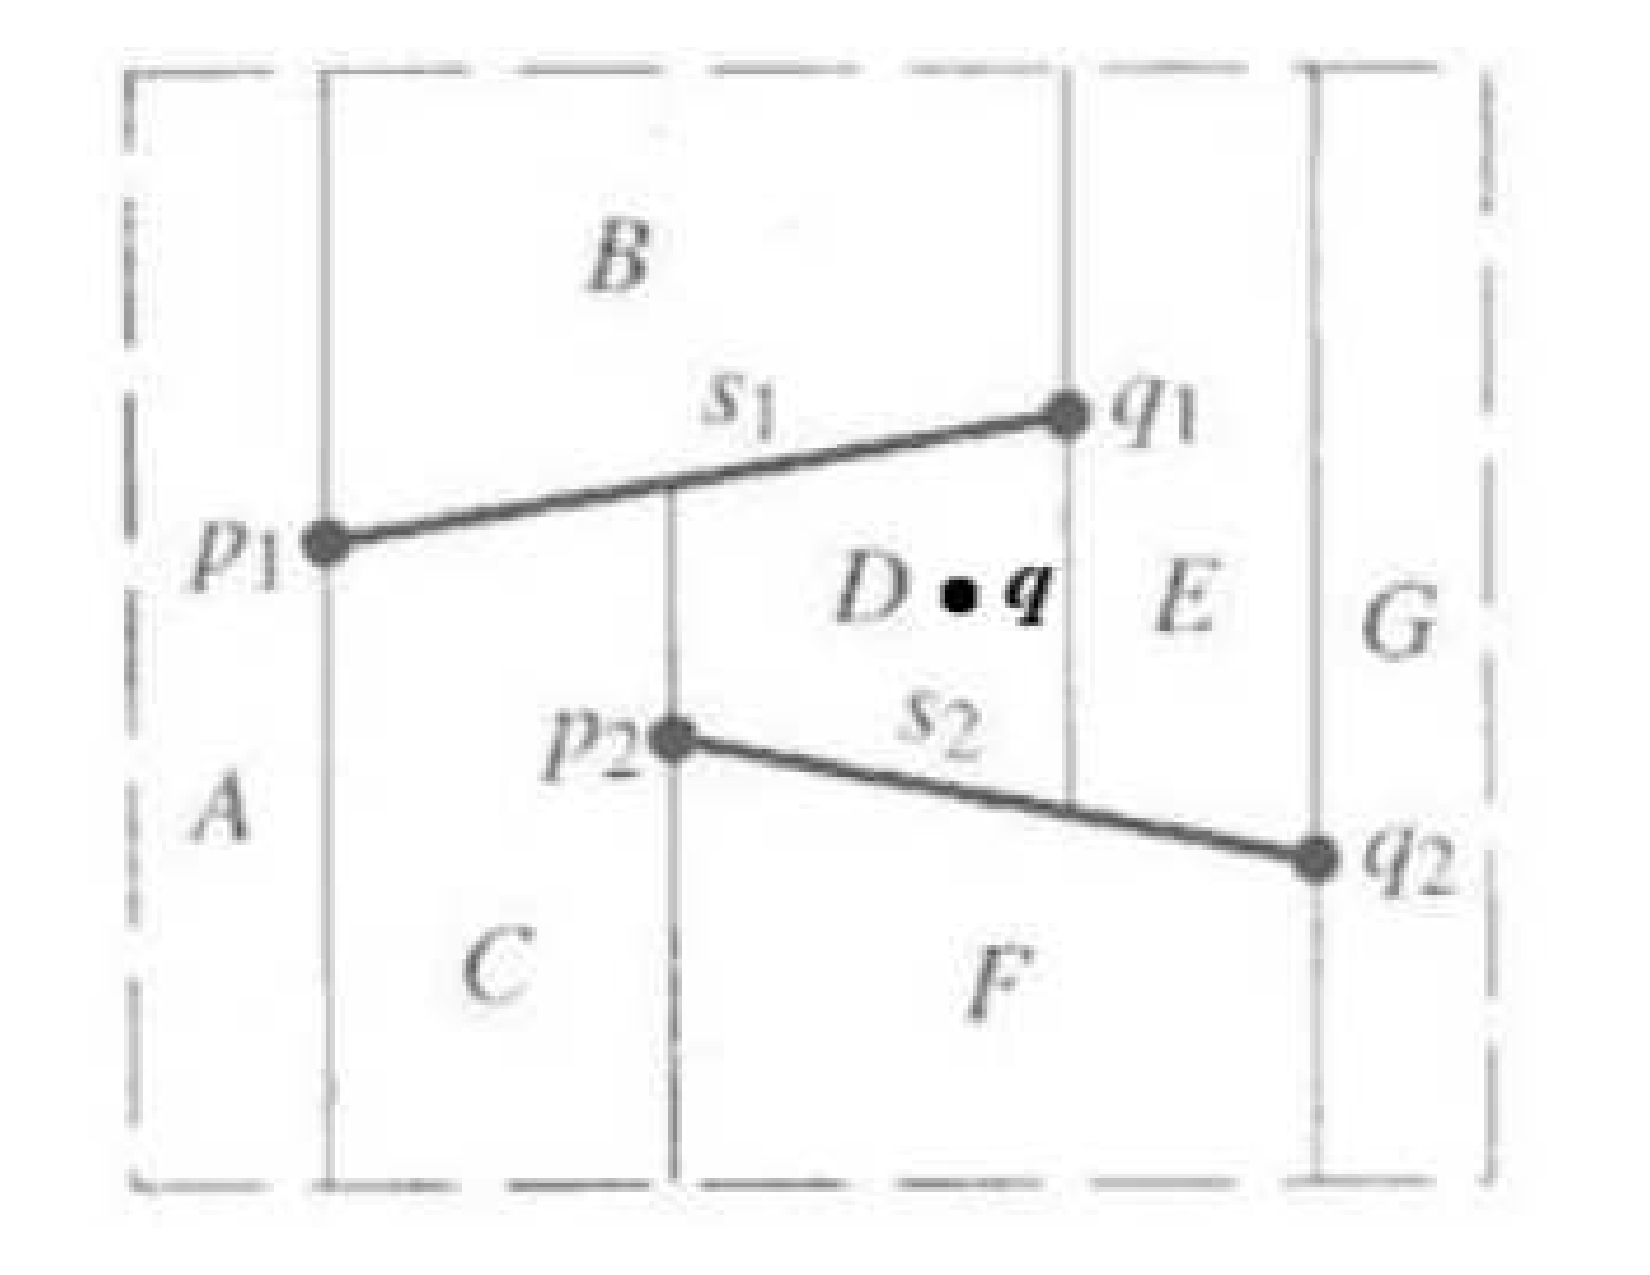
\includegraphics[width=50mm]{images/trapezoidal_map.pdf}
    \caption{A trapezoidal map inside a bounding box. Two line segments $s1$ and $s2$ have been inserted, which has generated a map of trapezoids $A$,$B$,$C$,$D$,$E$,$F$ and $G$. A query point $q$ is located in $D$.}
    \label{fig:trapezoidal_map}
\end{figure}

\subsubsection{Trapezoidal Map Algorithm}
The trapezoidal map algorithm takes as input a set of line segments forming a planar subdivision and outputs a trapezoidal map $T$ and a search tree $D$ that can be used to answer point location queries in O(logn) time. In return for the improved complexity, the algorithm will take O(nlogn) time to build the data structures. This is a desirable as we often want to perform several point location queries on the same map. 

\paragraph{}
Without modifications, the algorithm assumes that line segments are in general position. For a set of segments to be in general position they cannot cross each other (they can share an endpoint though) and no two distinct endpoints can lie on a vertical line.

\subsubsection{A trapezoidal map}
$T(S)$ of a planar subdivision represented as a list of segments S is created by erecting vertical lines (extensions) of each segment that stop when they hit an upper or lower segment. Each trapezoid of the resulting division will have one or two vertical sides and exactly two non-vertical sides. Since any vertical side of a trapezoid is created as an extension of an end point and no two endpoints can lie on a vertical line, a trapezoid can be uniquely represented as two points (left and right point) and two line segments (upper and lower boundaries). An example of a trapezoidal map can be seen in Figure~\ref{fig:trapezoidal_map}.

Two trapezoids are adjacent if the share a vertical side (an extension) and neighbours if they are adjacent and also share an upper or lower line segment. Any trapezoid in a trapezoidal map created from a set of line segments in general position can have at most 4 adjacent trapezoids and thereby at most 4 neighbours referred to as its upper left-, upper right-, lower left- and lower right neighbour. As an example, we can see in Figure~\ref{fig:trapezoidal_map} that the trapezoid $C$ has a $A$ as its lower left neighbour, $F$ as its lower right neighbour, and $D$ as its upper right neighbour.
\subsubsection{The search structure}
$D$ is a binary search tree that contains nodes representing the end point of a line segment (X nodes), the segment itself (Y nodes) or a trapezoid (leafs). Since the tree is assumed to be balanced (consult the references for an argument of why this is true), a trapezoid containing a query point can be found in O(logn) as a path from the root to a leaf. 

\begin{figure}[]
    \centering
      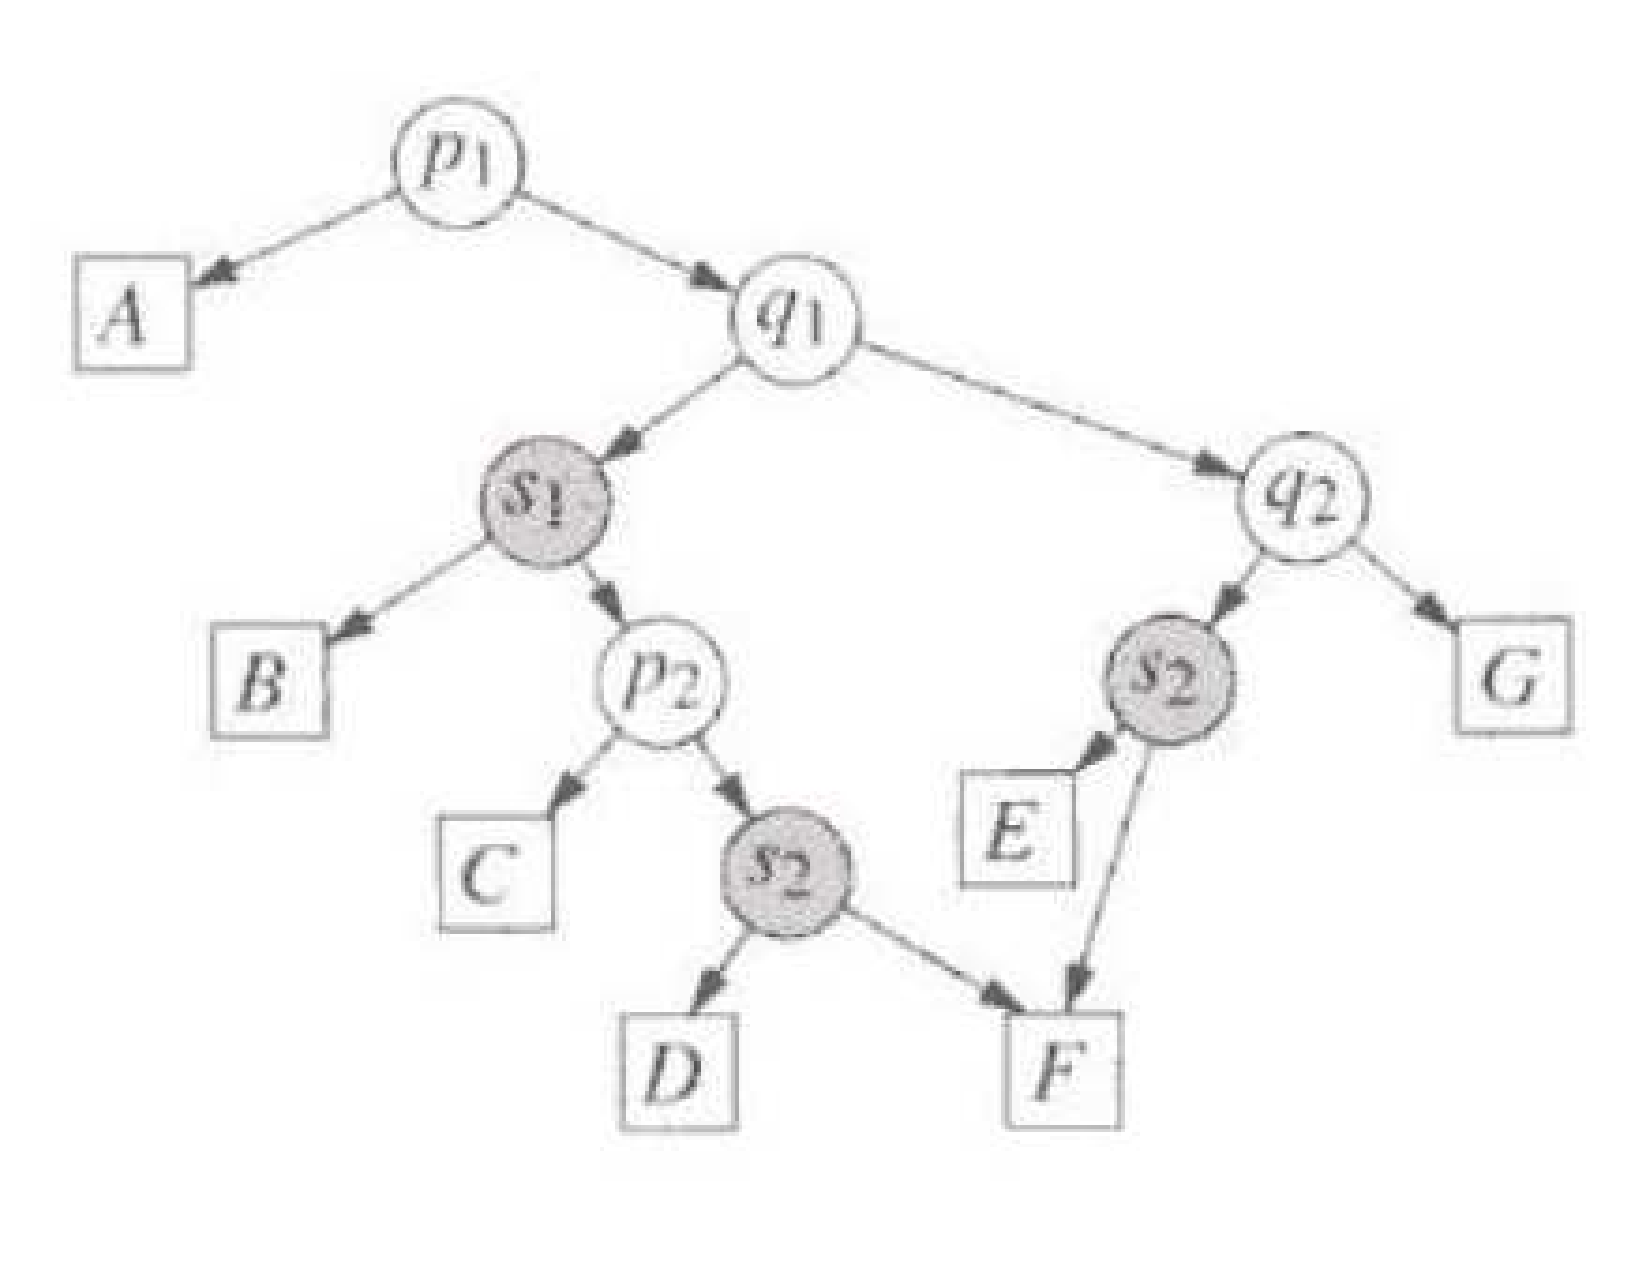
\includegraphics[width=80mm]{images/tree.pdf}
    \caption{A search tree with X nodes $p1$, $p2$, $p3$ and $p4$, Y nodes $s1$ and $s2$. The leaves are trapezoids $A$ to $G$. The search tree corresponds to the trapezodial map in Figure~\ref{fig:trapezoidal_map}.}
    \label{fig:tree}
\end{figure}

To find a path, one starts at the root and proceeds according to answers to questions varying with the type of node. At an X node, one proceeds in the left sub tree if the query point lies to the left of the end point that the node represents and right otherwise. At a Y node, one goes right if the query point lies below the line segment that the node represents and left otherwise.
The trapezoidal map algorithm is incremental in the sense that it starts with a blank map and a search tree containing only a single leaf (the rectangle or trapezoid that bounds the map). It then adds one edge to the map at a time and updates the search structures. To update the map, extensions are created from the end points of the newly added segment. If the segment intersects already existing extensions, these are shortened. To update the tree, the algorithm removes the leafs for the intersected trapezoids and adds leafs for the new ones that appear in the map.

In the case where a new segment is inserted and it spans multiple existing trapezoids, we have to create new trapezoids that may consist of merges of existing trapezoids. Using information about the neighbours, trapezoids can be merged in time linear in the number of trapezoids involved in the merge, which is assumed to be a constant operation. Furthermore,  the number of intersected trapezoids is not dependent on the number of segments in the input set. Updating therefore reduces to finding the left most intersected trapezoid. This can be done with a point location query in $D$ and the left most endpoint of the newly added line segment in O(logn) time. If the algorithm inserts $n$ segments, the global complexity of the algorithm will be O(nlogn)